\section{Technical acknowledgements}
\paragraph{}
The following code presented was written using \emph{Python 3.7}. The images from which the shapes were extracted were used as gray images. \ref{fig:gray-images}

\section{Loading data}
\begin{figure}
    \centering
    
\includegraphics[scale=2.0]{rdf-carre-6.png}
    
\includegraphics[scale=2.0]{rdf-carre-10.png}
    
\includegraphics[scale=2.0]{rdf-carre-10-30deg.png}
    
\includegraphics[scale=2.0]{rdf-triangle-10-15deg.png}
    
\includegraphics[scale=2.0]{rdf-triangle-10-45deg.png}
    
\includegraphics[scale=2.0]{rdf-triangle-10-60deg.png}
    
\includegraphics[scale=2.0]{rdf-triangle-20.png}
    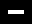
\includegraphics[scale=2.0]{rdf-rectangle-horizontal.png}
    
\includegraphics[scale=2.0]{rdf-rectangle-vertical.png}
    
\includegraphics[scale=2.0]{rdf-rectangle-diagonal.png}
    \caption{Shape images}
    \label{fig:gray-images}
\end{figure}

\paragraph{}
Images are loaded then converted to grayscale. Right now, we are not interested in their color.

\begin{lstlisting}[language=Python, caption=Loading images in Python]
def rdfReadGreyImage(nom):
    img = Image.open(f'images/{nom}').convert('L')
    img = np.asarray(img)
    return img
\end{lstlisting}

\clearpage

\section{Shape's main axis of inertia}
\subsection{Prerequisites}
\paragraph{}
We define the \emph{moment of a shape} as the following:
$$M_{ij} = \sum_{x}\sum_{y} x^{i} y^{j} A(x, y)$$
\paragraph{}
where $A(x, y)$ is the value of the pixel $(x, y)$ of the shape's image. One can easily observe that $M_{00}$ is equal to the number of pixels that are not black. We call that the \emph{surface} of the shape.

\begin{lstlisting}[language=Python, caption=Calculating the moment of a shape]
def rdfMoment(img, p, q):
    x = [x ** p for x in range(1, img.shape[0] + 1)]
    y = [y ** q for y in range(1, img.shape[1] + 1)]
    x, y = np.array(x), np.array(y)
    return np.dot(np.dot(x.T, img), y)
\end{lstlisting}

\paragraph{}
The \emph{barycentre} is defined as being the following:
$$(\bar{x}, \bar{y}) = (\frac{M_{10}} {M_{00}}, \frac{M_{01}} {M_{00}})$$

\paragraph{}
Having these, we can now make our $M_{ij}$ invariant to the rotation and translation of the shape. We can define the \emph{centered moment} as being:
$$\mu_{ij} = \sum_{x}\sum_{y} (x - \bar{x})^i(y - \bar{y})^j I(x, y)$$


\begin{lstlisting}[language=Python, caption=Calculating centered moments]
def rdfMomentCentre(img, p, q):
    # Barycentre
    s = rdfSurface(img)
    cx = rdfMoment(img, 1, 0) / s
    cy = rdfMoment(img, 0, 1) / s
    # Initialiser les vecteurs x et y
    x = [(x-cx) ** p for x in range(1, img.shape[0] + 1)]
    y = [(y-cy) ** q for y in range(1, img.shape[1] + 1)]
    # Calcul du moment centre
    return np.dot(np.dot(x, img), y)
\end{lstlisting}

\paragraph{}
And for our last trick, we can make $\mu_{ij}$ invariant to the scale of the image! We define the \emph{normalized centered moment} as the following:
$$\eta_{ij} = \frac{\mu_{ij}}{\mu_{00}^{1 + \frac{i + j}{2}}}$$

\begin{lstlisting}[language=Python, caption=Calculating normalised centered moments]
def rdfMomentCentreNormalise(img, p, q):
    upq = rdfMomentCentre(img, p, q)
    u00 = rdfMomentCentre(img, 0, 0)
    normalised = upq / (u00 ** (1 + (p + q)/2))
    return normalised
\end{lstlisting}

\subsection{Main axis of inertia}
\paragraph{}
Inspiring ourselves from physics, we may use the shape's moment of inertia matrix. With that, we're able to tell which is a figure's main axis of inertia.

\begin{lstlisting}[language=Python, caption=Calculating normalised centered moments]
def mainInertionAxis(img, normalise=True):
    f = rdfMomentCentreNormalise if normalise is True else rdfMomentCentre
    u20 = f(img, 2, 0)
    u11 = f(img, 1, 1)
    u02 = f(img, 0, 2)
    I = np.ndarray(buffer=np.array(
        [u20, u11, u11, u02]), shape=(2, 2), dtype='float')
    _, eigenVectors = np.linalg.eig(I)
    P = eigenVectors.T
    return P
\end{lstlisting}

\paragraph{}
Our first experiment is calculating the main axis for the 3 rectangles, in the following order: diagonal, horizontal and vertical. The results clearly show us that we can easily differentiate the fact that the shapes are rotated.
\begin{figure}[H]
    \centering
    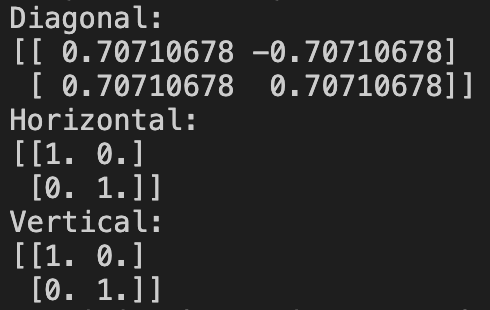
\includegraphics{main_axis_rectangles.png}
    \label{fig:main-axis-rectangles}
\end{figure}

\paragraph{}
Let us now analyse the square images. From the results, we can see that the main axis of inertia for the squares that only differ in size is the same.
For the square that is rotated, we get different results. Therefore, calculating the main axis of inertia is invariant to the scale of the shape.
\begin{figure}[H]
    \centering
    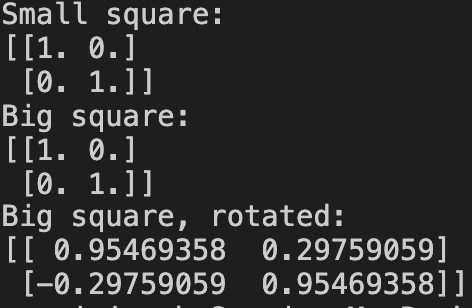
\includegraphics{main_axis_squares.png}
    \label{fig:main-axis-squares}
\end{figure}

% \begin{figure}
%     \begin{subfigure}
%         \centering
%         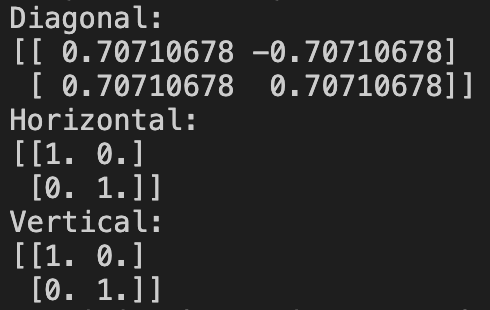
\includegraphics{main_axis_rectangles.png}
%         \label{fig:main-axis-rectangles}
%     \end{subfigure}

%     \begin{subfigure}
%         \centering
%         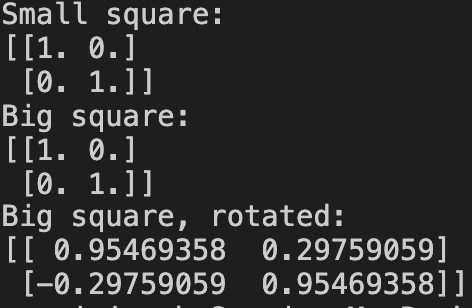
\includegraphics{main_axis_squares.png}
%         \label{fig:main-axis-squares}
%     \end{subfigure}
% \end{figure}